\section{Menú principal}

  \begin{figure}[H]
    \centering
    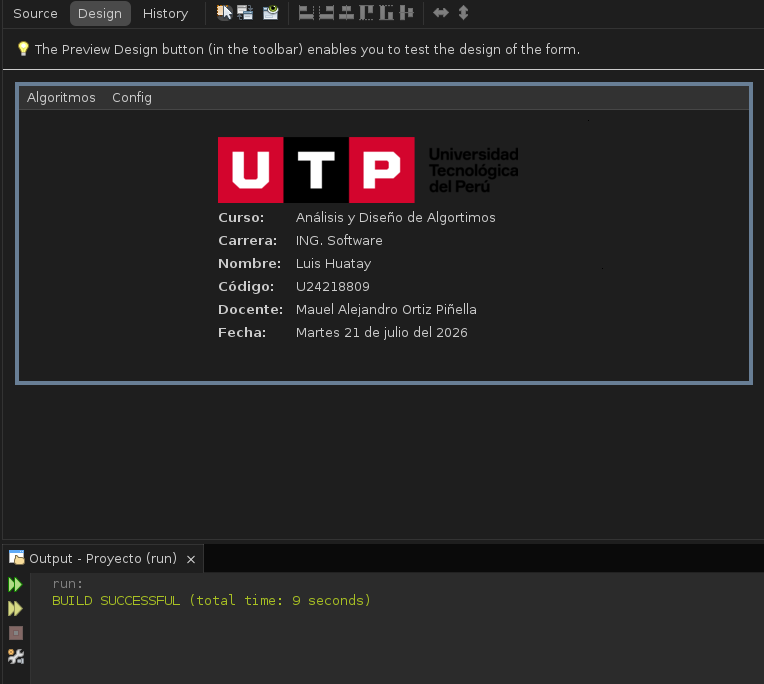
\includegraphics[width=1\textwidth]{assets/imgs/menu_build.png}
    \caption{Construcción del Menú con JFrame Form.}
  \end{figure}

  \begin{figure}[H]
    \centering
    
\includegraphics[width=1\textwidth]{assets/imgs/menu.png}
    \caption{Interfaz Menú.}
  \end{figure}

\section{Interfaz de Agenad de Mascotas}

  \begin{figure}[H]
    \centering
    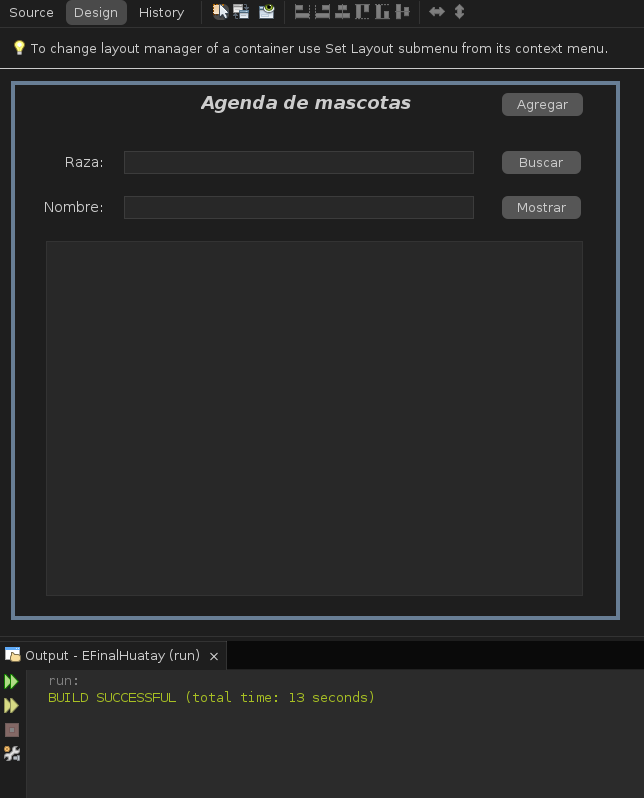
\includegraphics[width=0.7\textwidth]{assets/imgs/agendaBuild.png}
    \caption{Diseño de la interfaz de Agenda de Mascotas.}
  \end{figure}

  \begin{figure}[H]
    \centering
    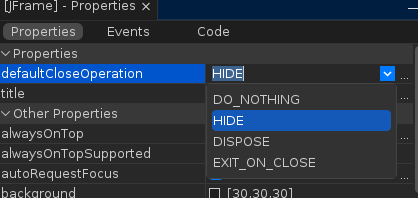
\includegraphics[width=0.7\textwidth]{assets/imgs/mergePropiedad.png}
    \caption{Propiedad que evita que se termine el programa al cerrar la ventana de Agenda de Mascotas.}
  \end{figure}

  \begin{figure}[H]
    \centering
    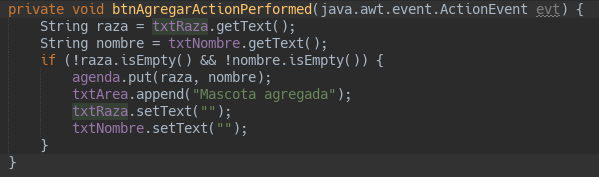
\includegraphics[width=0.9\textwidth]{assets/imgs/metodoAgregar.png}
    \caption{Método para agregar los datos de la mascota a la Agenda.}
  \end{figure}

  \begin{figure}[H]
    \centering
    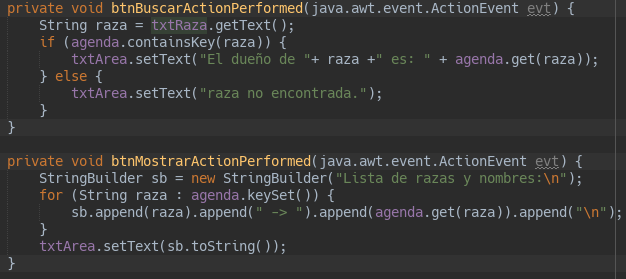
\includegraphics[width=0.9\textwidth]{assets/imgs/metodoBuscar.png}
    \caption{Método para buscar y mostrar los datos de la mascota en la Agenda.}
  \end{figure}

  \begin{figure}[H]
    \centering
    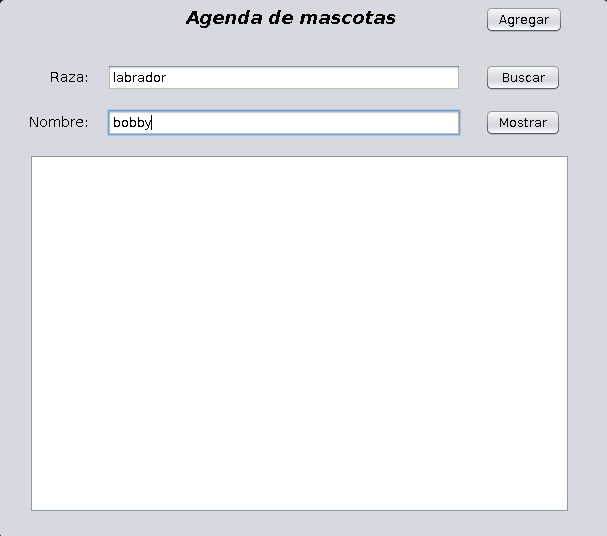
\includegraphics[width=0.9\textwidth]{assets/imgs/interfazMascota.png}
    \caption{Interfaz de la aplicación de Agenda de Mascotas, agregando 10 registros.}
  \end{figure}

  \begin{figure}[H]
    \centering
    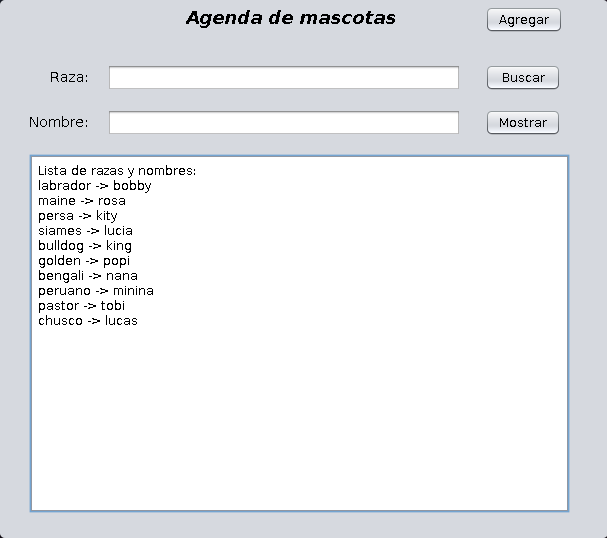
\includegraphics[width=0.9\textwidth]{assets/imgs/mascotasRegistros.png}
    \caption{Muestra de los registros de la Agenda de Mascotas.}
  \end{figure}

  \newpage

  \section{Interfaz de ordenamiento alfabético}

  \begin{figure}[H]
    \centering
    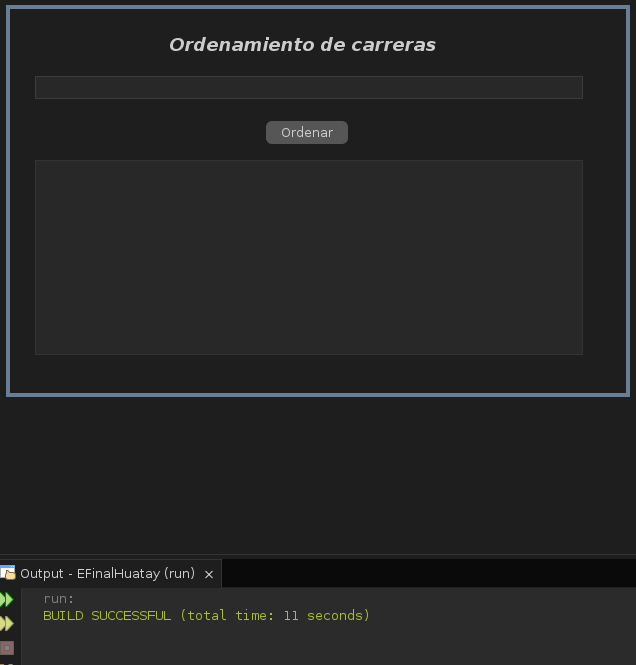
\includegraphics[width=0.8\textwidth]{assets/imgs/sortDise.png}
    \caption{Diseño de la interfaz de ordenamiento alfabético.}
  \end{figure}

  \begin{figure}[H]
    \centering
    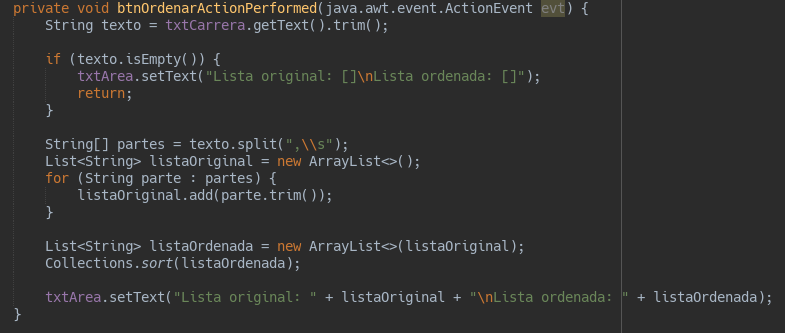
\includegraphics[width=0.9\textwidth]{assets/imgs/metodoSort.png}
    \caption{Método para ordenar los datos alfabéticamente.}
  \end{figure}

  \begin{figure}[H]
    \centering
    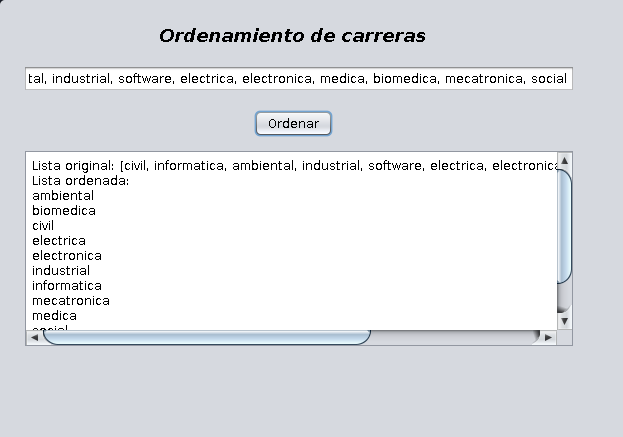
\includegraphics[width=0.9\textwidth]{assets/imgs/sortOrdenado.png}
    \caption{Muestra del funcionamiento de la interfaz de ordenamiento alfabético con los datos del examen.}
  \end{figure}

  \newpage

\section{Interfaz de Merge-Sort ascendente y descendente}

\begin{figure}[H]
    \centering
    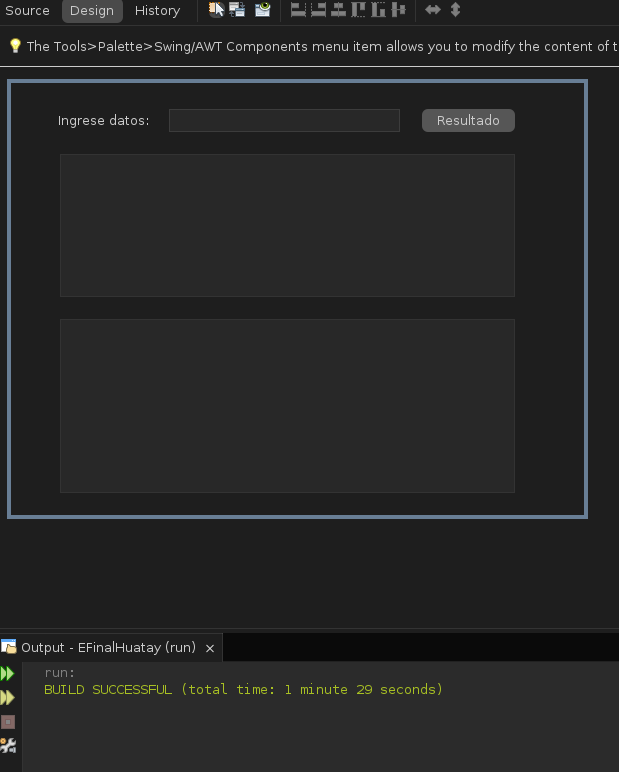
\includegraphics[width=0.7\textwidth]{assets/imgs/mergeDiseño.png}
    \caption{Diseño de la interfaz de Merge-Sort.}
  \end{figure}

  \begin{figure}[H]
    \centering
    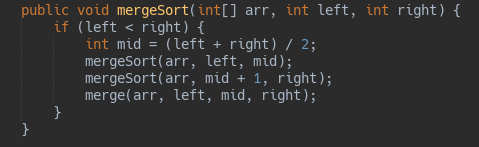
\includegraphics[width=0.7\textwidth]{assets/imgs/metodoMerge.png}
    \caption{Método para ordenar los datos del examen con Merge-Sort de manera recursiva.}
  \end{figure}

  \begin{figure}[H]
    \centering
    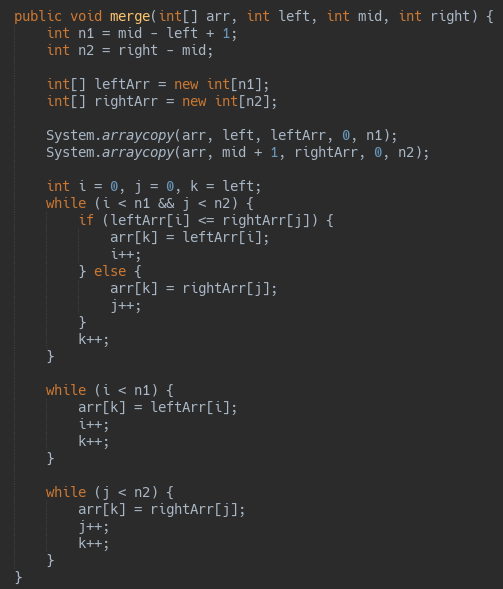
\includegraphics[width=0.7\textwidth]{assets/imgs/mergeLados.png}
    \caption{Método para unir los datos ordenados.}
  \end{figure}

  \begin{figure}[H]
    \centering
    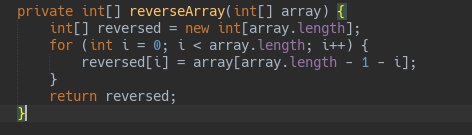
\includegraphics[width=0.7\textwidth]{assets/imgs/mergeReverse.png}
    \caption{Método para unir los datos ordenados en orden descendente.}
  \end{figure}

  \begin{figure}[H]
    \centering
    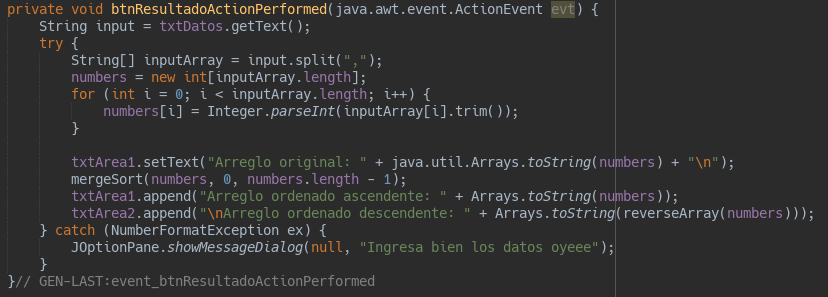
\includegraphics[width=0.9\textwidth]{assets/imgs/mergeLanzador.png}
    \caption{Comportamiento del botón de acción en la interfaz.}
  \end{figure}

  \begin{figure}[H]
    \centering
    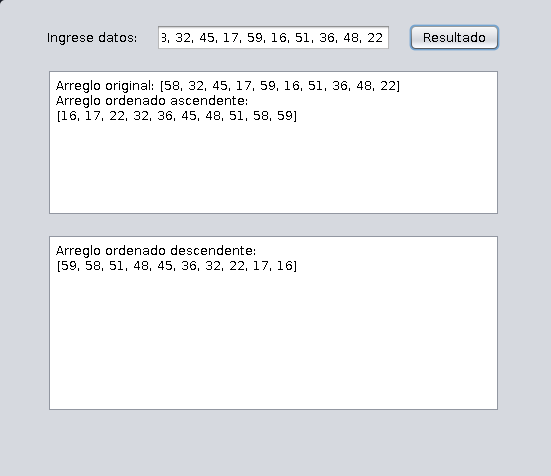
\includegraphics[width=0.8\textwidth]{assets/imgs/muestraMerge.png}
    \caption{Muestra del funcionamiento de la interfaz de Merge-Sort con los datos del examen.}
  \end{figure}
